\documentclass[11 pt]{article}
\usepackage[a4paper, total={6in, 8in}]{geometry}
\usepackage{float}
\usepackage{multirow}    % to add multirow cells in tables
\usepackage{indentfirst} %to automatically intent the first paragrap of each sections
\usepackage{amsmath}		%math packages
\usepackage{mathtools}
\usepackage{amssymb}
\usepackage{graphicx}	%Required for inserting images
\usepackage{fontenc}
\usepackage[colorlinks=true,linkcolor=blue,citecolor=blue, urlcolor=blue]{hyperref}	%for hyperlinks
\usepackage{subcaption}	%to add subcaptions within single floating enviroments
\usepackage{placeins}	%to control position of floating enviroments
\usepackage[numbers]{natbib}  %for correct formating of bibliography}\usepackage{import}
\usepackage[utf8]{inputenc}
\usepackage{tikz}
\usepackage{tikz-cd}
\usepackage{pgfplots}
\pgfplotsset{compat=1.14}
\bibliographystyle{abbrvnat}
\usepackage{siunitx} %for correct formating of units



\textwidth=170mm
\textheight=250mm
\hoffset= -20mm       % may need change
\voffset= -25mm       % may need change


\begin{document}

%% we do the title page ourselves
\thispagestyle{empty}     % only for frontpage
\null\vspace{40mm}
\begin{center}
{%%%%%%%%%%%%%%%%%%%%%%%%%% Titel
\Large  
Studying the $Z$ Boson with the ATLAS Detector at the LHC \footnote{\noindent Experiment FP94 perfomed the $4^{\textrm{th}}$ Nov. 2024. Supervisor:	Ruiz, Miguel}
}\\[15mm]
%%%%%%%%%%%%%%%%%%%%%%%%%%% Authors
Q. Coc and P. Huth

\vspace{25mm}

\parbox{0.9\textwidth}{
Abstract:    
\small 
In this experiment we measure the mass and width of the $Z$-Boson using pre-selected data measured by the ATLAS detector at the LHC in 2012. The data was compared to Monte Carlo simulations revealing data points generated by secondary processes which were filtered out. By fitting the convolution of a Gaussian and a Breit-Wigner distribution to filtered data we could determine $m_{Z} = \SI{90.629}{\mega\electronvolt}$ and $\Gamma = 3.258\pm 0.021$. Both values display a large deviation from the values reported by the Particle Data Group of $\sigma_{M_Z} = 27.11$ and $\sigma_{M_Z} = 36.09$.
}
\end{center}

\vfill
Als besondere Auswertung testiert: Datum, Unterschrift:
\vspace{20mm}

%% Rueckseite des Titelblatts leer. Bei einseitigem Druck entfernen
\newpage  
\null\thispagestyle{empty} 

\newpage
\section{Introduction}


\section{Selection of the data}
\begin{figure}[htbp]
    \centering
        \resizebox{0.7\textwidth}{!}{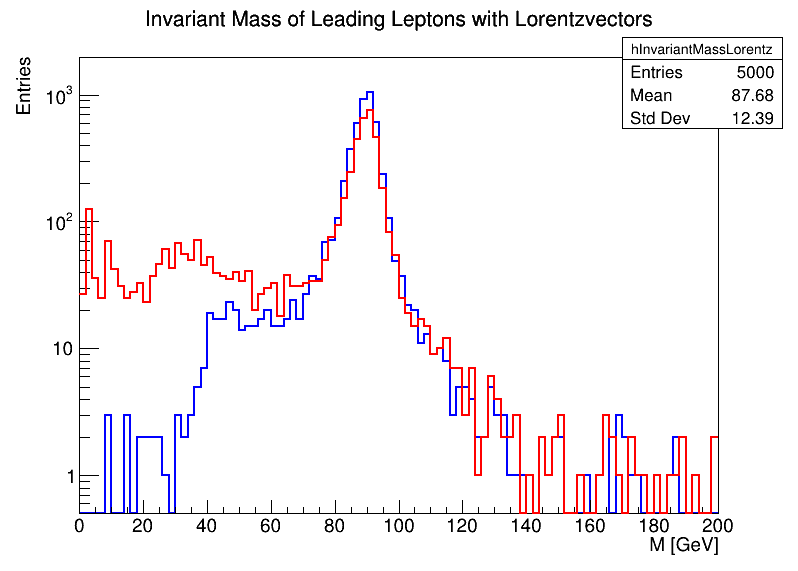
\includegraphics{Measurements/invariant_mass_comp_MC_log1.png}}
        \caption{Invariant mass from the measured events (red) compared to the invariant mass of Monte Carlo simulation (blue).}
        \label{fig:fit}
\end{figure}

\begin{figure}[htbp]
    \centering
    % First row
    \begin{subfigure}{0.45\textwidth}
        \centering
        \resizebox{0.8\textwidth}{!}{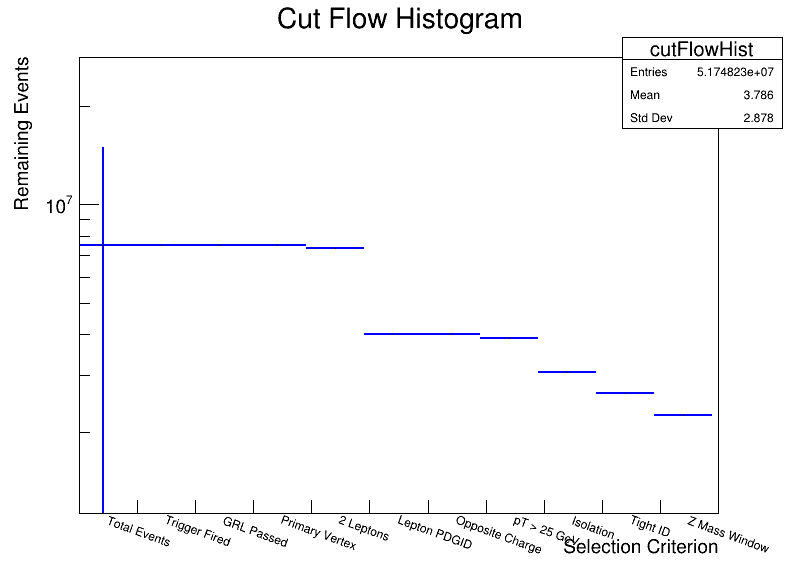
\includegraphics{Measurements/ZeecutFlowHist.png}}
        \caption{}
        \label{fig:sub1}
    \end{subfigure}
    \hfill
    \begin{subfigure}{0.45\textwidth}
        \centering
        \resizebox{0.8\textwidth}{!}{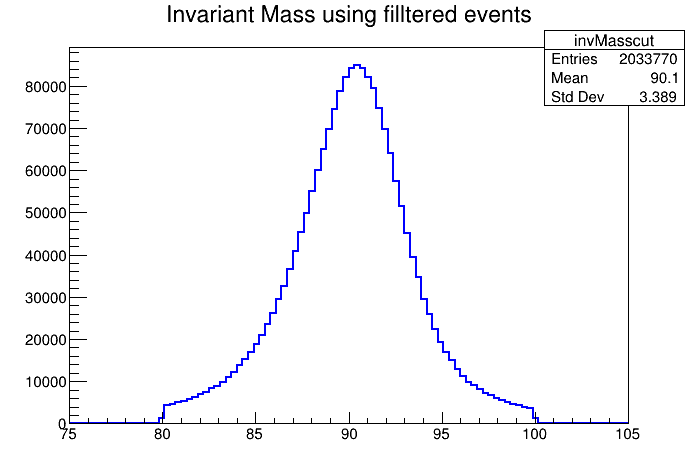
\includegraphics{Measurements/ZeeinvMass_cut.png}}
        \caption{}
        \label{fig:sub2}
    \end{subfigure}
\vspace{1em}
    \begin{subfigure}{0.45\textwidth}
        \centering
        \resizebox{0.8\textwidth}{!}{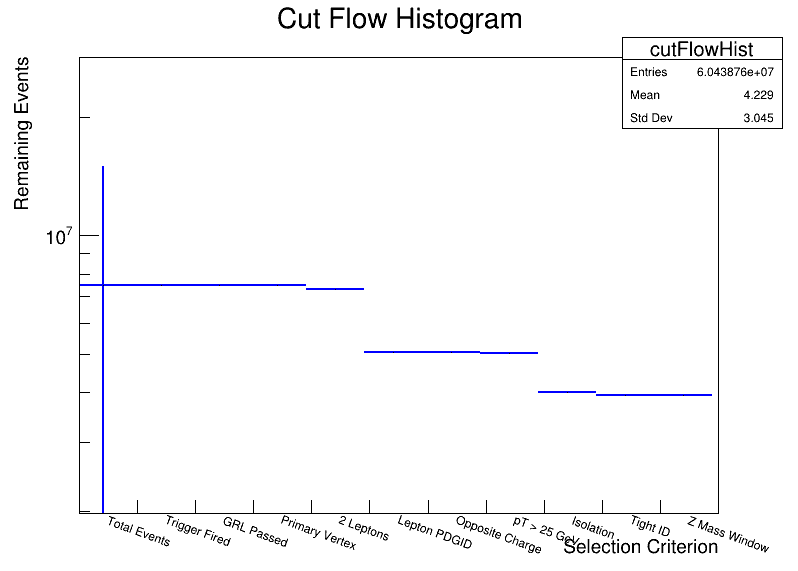
\includegraphics{Measurements/ZmumucutFlowHist.png}}
        \caption{}
        \label{fig:sub1}
    \end{subfigure}
    \hfill
    \begin{subfigure}{0.45\textwidth}
        \centering
        \resizebox{0.8\textwidth}{!}{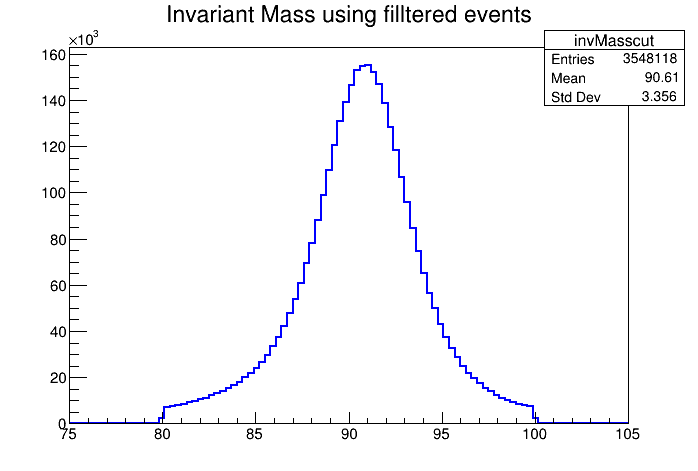
\includegraphics{Measurements/ZmumuinvMass_cut.png}}
        \caption{}
        \label{fig:sub2}
    \end{subfigure}
\vspace{1em}
    \begin{subfigure}{0.45\textwidth}
        \centering
        \resizebox{0.8\textwidth}{!}{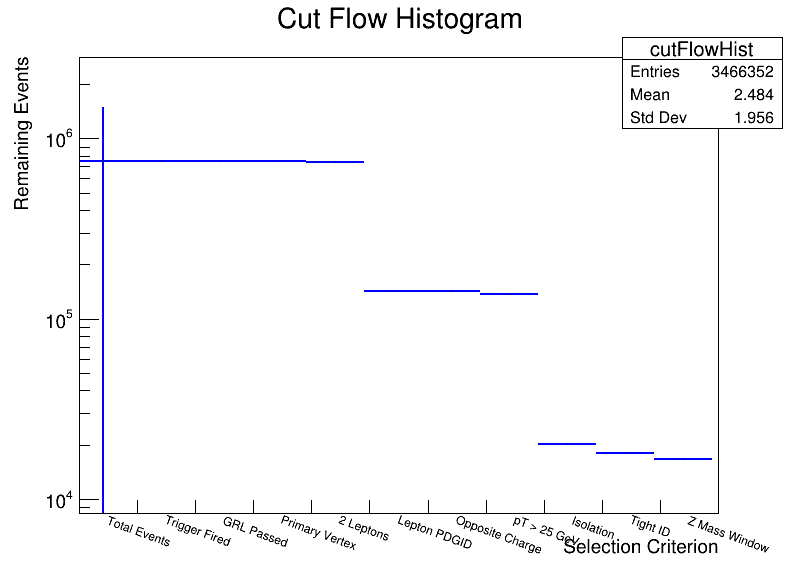
\includegraphics{Measurements/ZtautaucutFlowHist.png}}
        \caption{}
        \label{fig:sub1}
    \end{subfigure}
    \hfill
    \begin{subfigure}{0.45\textwidth}
        \centering
        \resizebox{0.8\textwidth}{!}{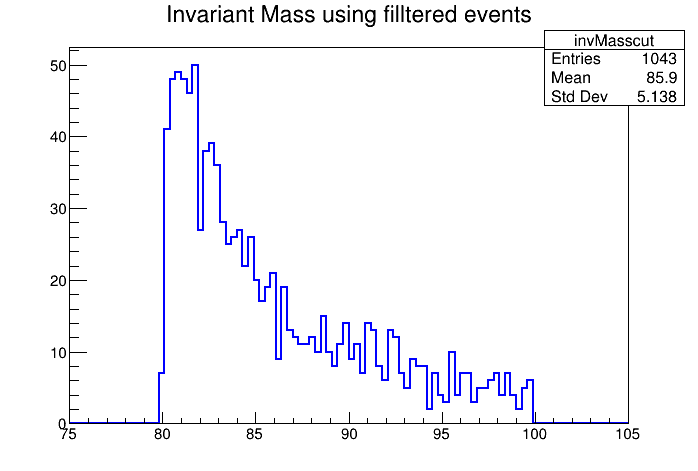
\includegraphics{Measurements/ZtautauinvMass_cut.png}}
        \caption{}
        \label{fig:sub2}
    \end{subfigure}
    \caption{\small Cut flow histograms from $e$, $\mu$ and $\tau$ events and the filtered events. In each row the cut flow histogram is display in the right while the events left after the selection process are presented on the right. The first row corresponds the events from $e$, the second from $\mu$ and the third one from $\tau$}
    \label{fig:selected_events}
\end{figure}

\section{Results}
\begin{figure}[htbp]
    \centering
        \resizebox{0.7\textwidth}{!}{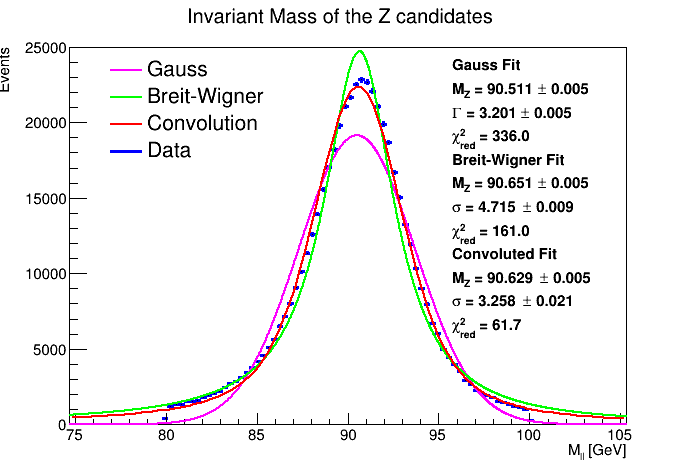
\includegraphics{Measurements/Fit.png}}
        \caption{\small Selected data (blue) and the fit of three distributions: (violet) Gauss-distribution, (green)Breit-Wigner Distribution and (red) convolution of a Gauss and Breit-Wigner distribution.}
        \label{fig:fit}
\end{figure}

\section{Discussion}
\end{document}